\documentclass[12pt]{article}
\textwidth = 15cm \oddsidemargin = 1.5cm \topmargin = -3cm \textheight = 21cm
%%\usepackage[russian]{babel}
\usepackage{feynmf}
\usepackage{amsmath} %% подключение математического пакета
%\usepackage{epstopdf}
%\usepackage{graphicx}
\usepackage{graphics}
\unitlength=1mm
%\documentstyle[12pt]{article}
%\renewcommand{\textheight}{22 cm}
%\renewcommand{\textwidth}{16 cm}
%\oddsidemargin 0cm \addtolength\topmargin{-2cm}

% DEFINITIONS
\def\eps{\varepsilon}
\def\epsilon{\varepsilon}
\def\Dm{\widetilde{\cal D}_{\mu}}
\def\const{{\rm const\,}}
\def\D{{\cal D}}
\def\L{{\cal L}}
\def\A{{\cal A}}
\def\S{{\cal S}}
\def\x{{\bf x}}
\def\p{{\bf p}}
\def\k{{\bf k}}
\def\q{{\bf q}}
\def\r{{\bf r}}
\def\h{{\bf h}}
\def\n{{\bf n}}
\def\bfx{{\bf x}}
\def\bfv{{\bf v}}
\def\bfu{{\bf u}}
% END OF DEFINITIONS

\begin{document}

\section{Introduction} \label{sec:Intro}



\section{Description of the models. Field theoretic formulation}
\label{sec:QFT}

In the Langevin formulation the models are defined by stochastic
differential equations for the order parameter
$\psi = \psi(t,{\bf x})$:
\begin{eqnarray}
\partial_{t} \psi_{a} = \lambda_{0} \left\{ (-\tau_{0} +
\partial^{2}) \psi_{a} - V(\psi) \right\} + \zeta  = 0,
\label{stoh}
\end{eqnarray}
where $\partial_{t}= \partial/ \partial t$, $\partial^{2}$ is the
Laplace operator, $\lambda_{0}>0$ is the kinematic (diffusion)
coefficient and $\tau_{0} \propto (T-T_{c})$ is the deviation of
the temperature (or its analog) from the critical value.
 The Gaussian random noise
$\zeta=\zeta(t,{\bf x})$ with the zero mean is specified by the
pair correlation function:
\begin{eqnarray}
\langle \zeta (t,{\bf x})\zeta (t',{\bf x'}) \rangle =
2 \lambda_{0}  \delta(t-t')\delta^{(d)}({\bf x}-{\bf x}')
\label{kor1}
\end{eqnarray}
 $d$ is the dimension of the ${\bf x}$ space.  Here and below, the bare (unrenormalized) parameters are
marked by the subscript ``o''. Their renormalized analogs (without
the subscript) will appear later on.  The
nonlinearity has the form $V(\psi)=g_{0}R_{abc} \psi_{b}(x)\psi_{c}(x)/2$; $g_{0}$
 being the coupling constant. Summations over repeated indices are always implied.
The tensor $R_{abc}$ is expressed in the terms of the set of $n+1$ vectors $e_{\alpha}$.
\begin{eqnarray}
R_{abc}=\sum\limits_{\alpha}e^{\alpha}_{a}e^{\alpha}_{b}e^{\alpha}_{c},
\label{Rofe}
\end{eqnarray}
where the $e_{a}^{\alpha}$ satisfy
\begin{eqnarray}
\sum\limits_{\alpha=1}^{n+1}e^{\alpha}_{a}=0,\quad \sum\limits_{\alpha=1}^{n+1}e^{\alpha}_{a}e^{\alpha}_{b}=(n+1)\delta_{ab},\quad \sum\limits_{\alpha=1}^{n}e_{a}^{\alpha}e_{a}^{\beta}=(n+1)\delta^{\alpha\beta}-1.
\label{esat}
\end{eqnarray}
Where $n$ is dimension of hyperspace. Using (\ref{esat}) one can obtain that contraction of two and three tensors R have forms
\begin{eqnarray}
R_{abc}R_{abd}=R_1\delta_{cd}, \quad R_{abc}R_{cde}R_{efa}=R_2 R_{bdf},
\label{rcont}
\end{eqnarray}
where
\begin{eqnarray}
R_1=(n+1)^2(n-1),\quad R_2=(n+1)^2(n-2).
\label{r1r2}
\end{eqnarray}



This stochastic problem (\ref{stoh}), (\ref{kor1}) can be
reformulated as field theoretic model of the
doubled set of fields $\Phi = \{\psi,\psi^{\dag}\}$ with action functional
\begin{eqnarray}
\S(\psi,\psi^{\dag}) =  \psi_{a}^{\dag}
\left(-\partial_{t}+\lambda_{0} \partial^{2}- \lambda_{0}\tau_{0}\right)
\psi_{a} + \lambda_{0} \psi_{a}^{\dagger}\psi_{a}^{\dagger} - g_{0}R_{abc}\lambda \psi^{\dag}_{a}\psi_{b}\psi_{c}/2.
\label{action}
\end{eqnarray}
Here, $\psi^{\dag}=\psi^{\dag}(t,{\bf x})$ is the auxiliary ``response
field'' and the integrations over the arguments of the fields are implied,
for example
\[  \psi^{\dag}\partial_{t}\psi = \int dt \int d{\bf x}
\psi^{\dag}(t,{\bf x})\partial_{t}\psi(t,{\bf x}). \]
The field theoretic formulation means that the statistical averages
of random quantities in the original stochastic problems can be represented
as functional integrals over the full set of fields with weight
$\exp {\cal S}(\Phi)$, and can therefore be viewed as the Green functions
of the field theoretic models with actions (\ref{action}).
In particular, the linear response function of the problems
(\ref{stoh}), (\ref{kor1}) is given by the Green function
\begin{eqnarray}
G=\langle \psi^{\dag}(t, {\bf x}) \psi(t', {\bf x'} ) \rangle =
\int {\cal D}\psi^{\dag} \int {\cal D} \psi\ \,
\psi^{\dag}(t, {\bf x}) \psi(t', {\bf x'})\, \exp {\cal S}(\psi,\psi^{\dag})
\label{respd}
\end{eqnarray}
of the corresponding field theoretic model.

The model (\ref{action}) corresponds to the standard Feynman
diagrammatic technique with two bare propagators
$\langle \psi \psi^{\dag} \rangle_{0}, \quad \langle \psi \psi \rangle_{0}$ and  triple vertex
$\sim \psi^{\dagger}\psi^2$.
In the frequency-momentum representation the propagators
have the forms
\begin{eqnarray}
\langle \psi \psi^{\dag} \rangle_{0} (\omega,k) =
\frac{1}{-{\rm i}\omega+\lambda_{0} \left(k^{2}+\tau_{0}\right)}, \nonumber \\
\langle \psi \psi \rangle_{0}(\omega,k) =
\frac{2\lambda_{0}}{\omega^2+\lambda_{0}^2 \left(k^{2}+\tau_{0}\right)^2}
\label{lines}
\end{eqnarray}


The Galilean invariant coupling with the velocity field
${\bf v}= \{ v_{i}(t,\bfx) \}$ for the compressible fluid
($\partial _i v_{i} \ne 0$) can be introduced by the replacement
\begin{eqnarray}
\partial_{t}\psi_{b} \to \partial_{t}\psi_{b} + a_{0}\, \partial_{i}(v_{i}\psi_{b}) +
(a_{0}-1) (v_{i} \partial_{i})\psi_{b} =
\nabla_{t} \psi_{b} + a_{0}(\partial_{i}v_{i}) \psi_{b}
\label{nabla}
\end{eqnarray}
in (\ref{stoh}). Here $\nabla_{t} \equiv \partial_{t} + v_{i} \partial_{i}$
is the Lagrangian derivative, $a_{0}$ is an arbitrary parameter and
$\partial_i = \partial /\partial x_{i}$. 

In the real problem, the field ${\bf v}(t,{\bf x})$ satisfies the
Navier--Stokes equation. We will employ the rapid-change model \cite{FGV},
where the velocity obeys a Gaussian distribution with zero mean and
the correlation function
\begin{eqnarray}
\langle v_{i}(t, \bfx) v_{j}(t',{\bf x'})\rangle =  \delta(t-t')\,
D_{ij}(\bf r), \quad \bf r = \bf x-{\bf x'}
\label{white}
\end{eqnarray}
with
\begin{eqnarray}
D_{ij}(\bf {r}) = D_{0}\, \int_{k>m} \frac{d{\bf {k}}}{(2\pi)^{d}} \,
\frac{1}{k^{d+\xi}}\, \left\{ P_{ij}({\bf k})+\alpha Q_{ij}({\bf
k}) \right\}\, \exp ({\rm i} {\bf {kr}} ).
\label{Kraich}
\end{eqnarray}
Here $P_{ij}({\bf k}) = \delta_{ij} - k_i k_j / k^2$ and
$Q_{ij}({\bf k})=k_i k_j/k^2$ are the transverse and the longitudinal
projectors, $k\equiv |{\bf k}|$ is the wave number,
$D_{0}>0$ is an amplitude factor and $\alpha>0$ is an arbitrary
parameter. The case $\alpha=0$ corresponds to the incompressible fluid
($\partial _i v_{i}=0$), while the limit $\alpha \to\infty$ at fixed
$\alpha D_{0}$ corresponds to the purely potential velocity field.
The exponent $0<\xi<2$ is a free parameter which can be viewed as a kind
of H\"{o}lder exponent, which measures ``roughness'' of the velocity field;
the ``Kolmogorov'' value is $\xi=4/3$, while the ``Batchelor'' limit
$\xi\to2$ corresponds to smooth velocity. The cutoff in the
integral (\ref{Kraich}) from below at $k=m$, where $m\equiv 1/{\cal L}$ is
the reciprocal of the integral turbulence scale ${\cal L}$, provides IR
regularization. Its precise form is unimportant; the sharp cutoff is the
simplest choice for the practical calculations.

The action functional for the full set of fields
$\Phi = \left\{ \psi,\psi^{\dag},{\bf v} \right\}$ become
\begin{eqnarray}
\S(\Phi) = \psi^{\dag}_{a} \left\{
-\nabla_{t} + \lambda_{0}\left( \partial^{2}- \tau_{0}\right)
- a_{0} (\partial_{i}v_{i}) \right\} \psi_{a} + \\ \nonumber
 +\lambda_{0} \psi^{\dag}_{a}\psi^{\dag}_{a}
- \frac{g_{0}\lambda_{0}}{2}R_{abc} \psi^{\dag}_{a} \psi_{b}\psi_{c} +  \S(\bfv)
\label{Action}
\end{eqnarray}
This is obtained from (\ref{action}), by the replacement
(\ref{nabla}) and adding the term corresponding to the Gaussian averaging
over the field $\bfv$ with the correlator (\ref{white}), (\ref{Kraich}):
\begin{eqnarray}
\S(\bf{v}) = -\frac{1}{2} \int dt \int d{\bf {x}} \int d{\bf {x'}}
v_{i} (t,\bf{x}) D_{ij}^{-1}(\bf{r}) v_{j} (t, {\bf {x'}}),
\label{Sv}
\end{eqnarray}
where
\[ D_{ij}^{-1}(\bf{r}) \propto D_{0}^{-1} r^{-2d-\xi} \]
is the kernel of the inverse linear operation for the function
$D_{ij}(\bf{r})$ in (\ref{Kraich}).

In addition to (\ref{lines}), the Feynman diagrams for the model
(\ref{Action}) involve the propagator
$\langle vv \rangle_{0}$ specified by the relations (\ref{white}),
(\ref{Kraich}) and the new vertex
\begin{equation}
\psi^{\dag} v_{i} V_{i} \psi \equiv -
\psi^{\dag}\left\{ (v_{i}\partial_{i}) \psi + a_{0}(\partial_{i}v_{i})
\right\} \psi.
\label{Vertex}
\end{equation}
In the diagrams it corresponds to the vertex factor
\begin{equation}
V_{i} = - {\rm i} k_{i} - {\rm i} a_{0} q_{i},
\label{VertexF}
\end{equation}
where $k_{i}$ is the momentum argument of the field $\psi$ and
$q_{i}$ is the momentum of $v_{i}$.

Actual expansion parameter in the perturbation theory of the model is $u_{0}=g_{0}^2$, so
for the full model, the role of the coupling constants (expansion
parameters in the perturbation theory) is played by the three parameters
\begin{equation}
u_{0}=g_{0}^2  \sim \Lambda^{6-d}, \qquad
w_{0} = D_{0}/\lambda_{0} \sim \Lambda^{\xi},
\qquad w_{0}a_{0} \sim \Lambda^{\xi}.
\label{charges}
\end{equation}
The last relations, following from the dimensionality considerations
(more precisely, see the next section), define the typical UV momentum
scale $\Lambda$. From the relations (\ref{charges}) it follows that the
interactions $\psi^{\dagger}\psi_{a}\psi_{a}$ become logarithmic (the corresponding coupling
constant $u_{0}$ becomes dimensionless) at $d=6$.
Thus for the single-charge problems (\ref{action}),
the value $d=d_{c}=6$ is
the upper critical dimension, and the deviation $\varepsilon=4-d_{c}$ plays the
part of the formal expansion parameter in the RG approach: the critical
exponents are nontrivial for $\varepsilon>0$ and are calculated as series in
$\varepsilon$.

The additional interactions $\sim \psi^{\dag}_{a} v\partial \psi_{a} $
of the full model (\ref{Action})
become logarithmic at $\xi=0$. The parameter $\xi$ is not
related to the spatial dimension and can be varied independently. However,
for the RG analysis of the full problems it is important that
all the interactions become logarithmic at the same time. Otherwise, one
of them would be weaker than the others from the RG viewpoint and it would
be irrelevant in the leading-order IR behaviour. As a result, some of the
scaling regimes of the full model would be overlooked.
In order to study all possible scaling regimes and the crossovers between
them, we need a genuine three-charge theory, in which all the interactions
are treated on equal footing. Thus we will treat $\varepsilon$ and $\xi$ as
small parameters of the same order, $\varepsilon \propto \xi$.
Instead of the plain $\varepsilon$ expansion in the single-charge models,
the coordinates of the fixed points, critical dimensions
and other quantities will be calculated as double expansions in the
$\varepsilon$--$\xi$ plane around the origin, that is, around the point in which
all the coupling constants in (\ref{charges}) become dimensionless.
Similar situation was encountered earlier in various models of turbulence
and complex critical behaviour, e.g. \cite{AHH,Alexa,AIK,AIM,Sak}.


\section{Canonical dimensions, UV divergences and the renormalization}
\label{sec:Reno}


It is well known that the analysis of UV divergences is based on the analysis
of canonical dimensions (``power counting''); see e.g. \cite{Zinn,Book3}.
Dynamical models of the type (\ref{action}), in contrast to static ones, have
two independent scales: the time scale $T$ and the length scale $L$. Thus
the canonical dimension of any quantity $F$ (a field or a parameter) is
characterized by two numbers, the
frequency dimension $d_{F}^{\omega}$ and the momentum dimension $d_{F}^{k}$,
defined such that $[F] \sim [T]^{-d_{F}^{\omega}} [L]^{-d_{F}^{k}}$. These
dimensions are found from the obvious normalization conditions
\[ d_k^k=-d_{\bf x}^k=1,\ d_k^{\omega} =d_{\bf x}^{\omega }=0,\
d_{\omega }^k=d_t^k=0, \ d_{\omega }^{\omega }=-d_t^{\omega }=1 \]
and from the requirement
that each term of the action functional be dimensionless (with
respect to the momentum and frequency dimensions separately).
Then, based on $d_{F}^{k}$ and $d_{F}^{\omega}$,
one can introduce the total canonical dimension
$d_{F}=d_{F}^{k}+2d_{F}^{\omega}$ (in the free theory,
$\partial_{t}\propto\partial^{2}$), which plays in the theory of
renormalization of dynamical models the same role as
the conventional (momentum) dimension does in static problems;
see Chap.~5 of \cite{Book3}.
The canonical dimensions for the models (\ref{Action})
are given in table~\ref{table1}, including renormalized parameters (without
subscript ``o''), which will be introduced soon.
\begin{table}[h!]
\caption{Canonical dimensions of the fields and parameters in the model (\protect\ref{Action}).}
\label{table1}
\begin{center}
\begin{tabular}{|c|c|c|c|c|c|c|c|c|c|c|}
\hline
$F$          & $\psi$ & $\psi^\dagger$ & $v$ & $\lambda_0,\lambda$ & $\tau_0,\tau$ & $ m,\mu,\Lambda$ & $g_0^2$ & $\omega_0$ & $g^2,\omega,\alpha,a_0,a$ \\
\hline
$d_F^k$      & $\frac{d-2}{2}$ & $\frac{d+2}{2}$ & $-1$ & $-2$ & $2$ & $1$ & $2-d$ & $\xi$ & $0$ \\
\hline
$d_F^\omega$ & 0 & 0 & $1$ & $1$ & $0$ & $0$ & $2$ & $0$ & $0$ \\
\hline
$d_F$        & $\frac{d-2}{2}$ & $\frac{d+2}{2}$ & $1$ & $0$ & $2$ & $1$ & $6-d$ & $\xi$ & $0$ \\
\hline
\end{tabular}
\end{center}
\end{table}

As already discussed in the end of the previous section, the full model is
logarithmic (all the coupling constants are simultaneously dimensionless) at
$d=6$ and $\xi=0$. Thus the UV divergences in the Green functions manifest
themselves as poles in $\varepsilon = 6-d$, $\xi$ and, in general, their linear
combinations.

The total canonical dimension of an arbitrary 1-irreducible Green function
$\Gamma = \langle\Phi \cdots \Phi \rangle _{\rm 1-ir}$
is given by the relation \cite{Book3}
\begin{equation}
d_{\Gamma }=d_{\Gamma }^k+2d_{\Gamma }^{\omega }= d+2-N_{\Phi }d_{\Phi},
\label{dGamma}
\end{equation}
where $N_{\Phi}=\{N_{\psi},N_{\psi^{\dag}}, N_{v}\}$ are the numbers of
corresponding fields entering into the function $\Gamma$, and the summation
over all types of the fields is implied. The total dimension $d_{\Gamma}$
in logarithmic theory (that is, at $\varepsilon=\xi=0$) is the formal index of the
UV divergence $\delta_{\Gamma}=d_{\Gamma}|_{\varepsilon=\xi=0}$. Superficial UV
divergences, whose removal requires counterterms, can be present only in
those functions $\Gamma$ for which $\delta_{\Gamma}$ is a non-negative
integer.

From table~\ref{table1} and (\ref{dGamma}) we find
\begin{equation}
\delta_{\Gamma}= 8 - 2N_{\psi} - 4N_{\psi^{\dag}} - N_{v}.
\label{Inde}
\end{equation}


In dynamical models, the 1-irreducible diagrams without the fields
$\psi^{\dag}$ vanish, and it is sufficient to consider the functions
with $N_{\psi^{\dag}} \ge 1$. In our model we have Galilean symmetry and symmetry of
tensor $R_{acc}=0$ from (\ref{Rofe}),(\ref{esat}). With these restrictions, the analysis of
the expressions (\ref{Inde}) shows that in 
model, superficial UV divergences can be present in the following
1-irreducible functions:
\[ \langle \psi^{\dag} \psi^{\dag} \rangle \quad (\delta=0) \quad
{\rm with\ the\ counterterms} \quad \psi^{\dag}\psi^{\dag}, \]

\[ \langle \psi^{\dag} \psi \rangle \quad (\delta=2) \quad
{\rm with\ the\ counterterms} \quad \psi^{\dag}\partial_{t}\psi, \
\psi^{\dag}\partial^{2}\psi, \ \psi^{\dag}\psi, \]

\[ \langle \psi^{\dag} \psi \psi \rangle \quad (\delta=0) \quad
{\rm with\ the\ counterterms} \quad \psi^{\dag} \psi \psi, \]

\[ \langle \psi^{\dag} \psi v \rangle \quad (\delta=1) \quad
{\rm with\ the\ counterterms} \quad \psi^{\dag} (v\partial) \psi, \
\psi^{\dag} (\partial v) \psi.  \]


All the remaining terms are present in the corresponding action functional
(\ref{Action}), so that our models are multiplicatively
renormalizable. 
The Galilean symmetry also requires that the counterterms
$\psi^{\dag}\partial_{t}\psi$ and $\psi^{\dag} (v\partial) \psi $
enter the renormalized action only in the form of the Lagrangian
derivative $\psi^{\dag}\nabla_{t}\psi$, imposing no restriction on
the Galilean invariant term $\psi^{\dag} (\partial v) \psi $.


We thus conclude that the renormalized actions can be written in the forms
\begin{eqnarray}
\S^{R}(\Phi) =  \psi^{\dag}_{a} \left\{
- Z_{1} \nabla_{t} + \lambda\left( Z_{2} \partial^{2}- Z_{3}\tau\right)
- a Z_{6} (\partial_{i}v_{i}) \right\} \psi_{a}  + \\ \nonumber
+\lambda Z_{5}  \psi^{\dag}_{a}\psi^{\dag}_{a} -
gR_{abc}\mu^{\varepsilon} \lambda Z_{4}  \psi^{\dag}_{a}\psi_{b} \psi_{c} /2 +  \S(\bfv)
\label{ActionR}
\end{eqnarray}
for the model with $\S(\bfv)$ from (\ref{Sv}).

Here $\lambda$, $\tau$, $g$, $u$ and $a$ are renormalized analogs of the
bare parameters (with the subscripts ``o'') and $\mu$ is the reference mass
scale (additional arbitrary parameter of the renormalized theory). The
renormalization constants $Z_{i}$ absorb the poles in $\varepsilon$ and $\xi$ and
depend on the dimensionless parameters $u$, $w$, $\alpha$ and $a$.
Expression (\ref{ActionR}) can be reproduced by the
multiplicative renormalization of the fields $\psi \to \psi Z_{\psi}$,
$\psi^{\dag} \to \psi^{\dag} Z_{\psi^{\dag}}$
and the parameters:
\begin{eqnarray}
g_{0} = g \mu^{\varepsilon/2} Z_{g}, \quad u_{0} = g \mu^{\varepsilon} Z_{u}, \quad
w_{0} = w \mu^{\xi} Z_{w}, \nonumber \\
\lambda_{0} = \lambda Z_{\lambda}, \quad
\tau_{0} = \tau Z_{\tau},  \quad  a_{0} = a Z_{\tau}.
\label{Multy}
\end{eqnarray}

Since the last term $\S(\bfv)$ given by (\ref{Sv}) is not renormalized,
the amplitude $D_{0}$ from (\ref{Kraich}) is expressed in renormalized
parameters as $D_{0} = w_{0} \lambda_{0}  = w\lambda \mu^{\xi}$, while
the parameters $m$ and $\alpha$ are not renormalized: $m_{0} = m$,
$\alpha_{0} = \alpha$. Owing to the Galilean symmetry, the both terms
in the covariant derivative $\nabla_{t}$ are renormalized with the same
constant $Z_{1}$, so that the velocity field is not renormalized, either.
Hence the relations
\begin{eqnarray}
Z_{w}Z_{\lambda} =1, \quad Z_{m}= Z_{\alpha} = Z_{v} =1.
\label{RenD}
\end{eqnarray}
Comparison of the expressions (\ref{Action}) and
(\ref{ActionR}) gives the following relations between
the renormalization constants $Z_{1}$--$Z_{6}$ and (\ref{Multy}):
\begin{eqnarray}
Z_{1} = Z_{\psi} Z_{\psi^{\dagger}}, \quad Z_{2} = Z_{1}Z_{\lambda}, \quad
Z_{3} = Z_{2} Z_{\tau},\\ \nonumber Z_{4} = Z_{\lambda} Z_{\psi^{\dagger}}^{2}, \quad
Z_{5} = Z_{\lambda}Z_{g} Z_{\psi}^{3} Z_{\psi^{\dagger}}, \quad Z_{6} = Z_{1} Z_{a}
\label{ZZ}
\end{eqnarray}
for the Potts model.
Resolving these relations with respect to the renormalization constants
of the fields and parameters gives
\begin{eqnarray}
Z_{\lambda} = Z_{1}^{-1} Z_{2}, \quad Z_{\tau} = Z_{2}^{-1} Z_{3}, \quad
Z_{a} = Z_{1}^{-1} Z_{6}, \quad
Z_{u} = Z_{1}^{-1} Z_{2}^{-3} Z_{4}^{2} Z_{5}, \\ \nonumber 
Z_{\psi}= Z_{1}^{1/2}Z_{2}^{1/2}Z_{5}^{-1/2}, \quad
Z_{\psi}^{\dag}= Z_{1}^{1/2}Z_{2}^{-1/2}Z_{5}^{1/2}
\label{ResoC}
\end{eqnarray}
for the model, where we passed to the coupling
constant $u=g^{2}$ with $Z_{u}=Z_{g}^{2}$.


The renormalization constants can be found from the requirement that the
Green functions of the renormalized model
(\ref{ActionR}), when expressed in renormalized
variables, be UV finite (in our case, be finite at $\varepsilon\to0$,
$\xi\to0$). The constants $Z_{1}$--$Z_{6}$ are calculated directly from
the diagrams, then the constants in (\ref{Multy}) are found from
(\ref{ResoC}). In order to find the full set of constants,
it is sufficient to consider the 1-irreducible Green functions which involve
superficial divergences; In the one-loop approximation, they are given in this equations.

%%phi'phi'
\begin{eqnarray}
\begin{fmffile}{ds7dkfgs97ad}
\langle \psi^{\dag} \psi^{\dag} \rangle _{1-ir}= 2\lambda Z_{5} +
\parbox{30mm}{
\begin{fmfgraph*}(30,20)
\fmfright{i}
  \fmfleft{o}
  \fmfdot{v1,v2}
  \fmf{fermion,tension=3}{i,v1}
  \fmf{fermion,tension=3}{o,v2}
  \fmf{plain,right,left=0.7, tension=.5}{v2,v1}
  \fmf{plain,right,left=0.7, tension=.5}{v1,v2}
    \end{fmfgraph*}} +  \parbox{30mm}{\begin{fmfgraph*}(30,20)
 \fmfright{i}
  \fmfleft{o}
  \fmfdot{v1,v2}
  \fmf{fermion,tension=3}{i,v1}
  \fmf{fermion,tension=3}{o,v2}
  \fmf{plain,right,left=0.7, tension=.5}{v2,v1}
  \fmf{photon,right,left=0.7, tension=.5}{v1,v2}
   \end{fmfgraph*}}
\end{fmffile}
\end{eqnarray}

%%phi phi'
\begin{eqnarray}
\begin{fmffile}{ds1sgk7dfs97ad}
\langle \psi \psi^{\dag} \rangle _{1-ir}=  Z_{1} i\omega - \lambda\left( Z_{2} k^2- Z_{3}\tau\right)+
\parbox{30mm}{
\begin{fmfgraph*}(30,20)
\fmfright{i}
  \fmfleft{o}
  \fmfdot{v1,v2}
  \fmf{plain,tension=3}{i,v1}
  \fmf{fermion,tension=3}{o,v2}
  \fmf{fermion,right,left=0.7, tension=.5}{v2,v1}
  \fmf{plain,right,left=0.7, tension=.5}{v1,v2}
    \end{fmfgraph*}} +  \parbox{30mm}{\begin{fmfgraph*}(30,20)
 \fmfright{i}
  \fmfleft{o}
  \fmfdot{v1,v2}
  \fmf{plain,tension=3}{i,v1}
  \fmf{fermion,tension=3}{o,v2}
  \fmf{fermion,right,left=0.7, tension=.5}{v2,v1}
  \fmf{photon,right,left=0.7, tension=.5}{v1,v2}
   \end{fmfgraph*}}
\end{fmffile}
\end{eqnarray}




%%psi psi psidag
\begin{eqnarray}
\langle \psi\psi\psi^{\dag}\rangle _{1-ir} =
-g\lambda\mu^{\frac{\epsilon}{2}}Z_4+{
\parbox[c]{25mm}{\center\begin{fmffile}{sgff6dggif0}\begin{fmfgraph*}(20,35)
  \fmfright{r}
  \fmfleft{l}
  \fmftop{t}
  \fmfdot{v1,v2,v3}
  \fmf{plain,tension=3}{v2,r}
  \fmf{plain,tension=3}{v1,l}
  \fmf{plain,tension=.4}{v3,v2}
  \fmf{fermion,tension=.4}{v3,v1}
  \fmf{fermion,tension=.4}{v1,v2}
  \fmf{fermion,tension=3}{t,v3}
   \end{fmfgraph*}
   \end{fmffile}}}
   +\parbox[c]{25mm}{\center\begin{fmffile}{ddg7gf0}\begin{fmfgraph*}(20,35)
  \fmfright{r}
  \fmfleft{l}
  \fmftop{t}
  \fmfdot{v1,v2,v3}
    \fmf{plain,tension=3}{v2,r}
  \fmf{plain,tension=3}{v1,l}
  \fmf{fermion,tension=.4}{v3,v2}
  \fmf{fermion,tension=.4}{v3,v1}
  \fmf{photon,tension=.4}{v2,v1}
  \fmf{fermion,tension=3}{t,v3}
   \end{fmfgraph*}
   \end{fmffile}} +
 \parbox[c]{25mm}{\center\begin{fmffile}{8gsdg0}\begin{fmfgraph*}(20,35)
  \fmfright{r}
  \fmfleft{l}
  \fmftop{t}
  \fmfdot{v1,v2,v3}
  \fmf{plain,tension=3}{v2,r}
  \fmf{plain,tension=3}{v1,l}
  \fmf{fermion,tension=.4}{v3,v2}
  \fmf{fermion,tension=.4}{v3,v1}
  \fmf{plain,tension=.4}{v2,v1}
  \fmf{fermion,tension=3}{t,v3}
   \end{fmfgraph*}
   \end{fmffile}}
   \end{eqnarray}

%%psi psi psidag
\begin{eqnarray}
\langle \psi\psi^{\dag}v\rangle _{1-ir} =
-a_{0}k_{i}Z_6+{
\parbox[c]{25mm}{\center\begin{fmffile}{sgffgdgd6if0}\begin{fmfgraph*}(20,35)
  \fmfright{r}
  \fmfleft{l}
  \fmftop{t}
  \fmfdot{v1,v2,v3}
  \fmf{photon,tension=3}{v2,r}
  \fmf{plain,tension=3}{v1,l}
  \fmf{fermion,tension=.4}{v3,v2}
  \fmf{plain,tension=.4}{v3,v1}
  \fmf{fermion,tension=.4}{v2,v1}
  \fmf{fermion,tension=3}{t,v3}
   \end{fmfgraph*}
   \end{fmffile}}}
   +\parbox[c]{25mm}{\center\begin{fmffile}{d7fggfdgf0}\begin{fmfgraph*}(20,35)
  \fmfright{r}
  \fmfleft{l}
  \fmftop{t}
  \fmfdot{v1,v2,v3}
  \fmf{photon,tension=3}{v2,r}
  \fmf{plain,tension=3}{v1,l}
  \fmf{fermion,tension=.4}{v3,v2}
  \fmf{fermion,tension=.4}{v3,v1}
  \fmf{plain,tension=.4}{v2,v1}
  \fmf{fermion,tension=3}{t,v3}
   \end{fmfgraph*}
   \end{fmffile}} +
 \parbox[c]{25mm}{\center\begin{fmffile}{8gfgdggs0}\begin{fmfgraph*}(20,35)
  \fmfright{r}
  \fmfleft{l}
  \fmftop{t}
  \fmfdot{v1,v2,v3}
  \fmf{photon,tension=3}{v2,r}
  \fmf{plain,tension=3}{v1,l}
  \fmf{plain,tension=.4}{v3,v2}
  \fmf{fermion,tension=.4}{v3,v1}
  \fmf{fermion,tension=.4}{v1,v2}
  \fmf{fermion,tension=3}{t,v3}
   \end{fmfgraph*}
   \end{fmffile}}
   \end{eqnarray}



The solid lines with arrows denote the propagator $\langle \psi \psi^{\dag} \rangle_{0}$,
the arrow points to the field $\psi^{\dag}$. The solid lines without arrows
correspond to the propagator $\langle \psi \psi \rangle_{0}$ and the wavy lines denote the
velocity propagator $\langle vv \rangle_{0}$ specified in (\ref{white}).
The external ends with incoming arrows correspond to the fields
$\psi^{\dag}$, the ends without arrows correspond to $\psi$. The triple
vertex with one wavy line corresponds to the vertex factor (\ref{VertexF}).




All the diagrammatic elements should be expressed in renormalized variables
using the relations (\ref{Multy})--(\ref{ZZ}). In the one-loop approximation,
the $Z$'s in the bare terms should be taken in the first order in $u= g^{2}$
and $w$, while in the diagrams they should simply be replaced with unities,
$Z_{i} \to 1$. Thus the passage to renormalized variables in the diagrams
is achieved by the simple substitutions
$\lambda_{0} \to \lambda$, $\tau_{0} \to \tau$,
$g_{0} \to g\mu^{\varepsilon/2}$ and $w_{0} \to w\mu^{\xi}$.

In practical calculations, we used the minimal subtraction (MS) scheme,
in which the renormalization constants have the forms $Z_{i}=1+\,$ only
singularities in $\varepsilon$ and $\xi$, with the coefficients depending
on the completely dimensionless renormalized parameters $u$, $w$, $a$ and
$\alpha$. And results for $z_{i}$ have forms:
\begin{eqnarray}
Z_{1} = 1 - \frac{uR_{1}}{2\varepsilon}, \quad
Z_{2} = 1 - \frac{uR_{1}}{3\varepsilon} - \frac{w}{6\xi}(5+\alpha), \quad
Z_{3} = 1 - \frac{2R_{1}u}{\varepsilon}, \nonumber \\
Z_{4} = 1 - \frac{2R_{2}u}{\varepsilon} - \frac{w \alpha a^2}{\xi}, \quad
Z_{5} = 1 - \frac{uR_{1}}{2\varepsilon} - \frac{w}{\xi} \alpha (a-1)^{2}, \nonumber \\
Z_{6} = 1 - \frac{uR_{1}}{\varepsilon 2a}(4a-1). 
\label{Zo}
\end{eqnarray}
To simplify the resulting expressions, we passed in (\ref{Zo})
 to the new parameters
\[ u \to u/128\pi^3, \quad w \to w/64\pi^3; \]
here and below they are denoted by the same symbols $u$ and $w$.
The parameters $R_{1}$ and $R_{2}$ are related to the dimension $n$ of the order parameter by the 
expression (\ref{r1r2}). Although we are especially interested in the cases $n=0$ and $n=-1$,
for completeness the coefficients $R_{1}$ and $R_{2}$ in  what follows are assumed to be arbitrary.

These relations will play an important role in the analysis of the
fixed points of the model (\ref{Action}) in the next sections.


\section{RG functions and RG equations} \label{sec:RGE}

Let us recall an elementary derivation of the RG equations; detailed
exposition can be found in monographs \cite{Zinn,Book3}.
The RG equations are written for the renormalized Green functions
$G^{R} =\langle \Phi\cdots\Phi\rangle_{R}$, which differ from the original
(unrenormalized) ones $G =\langle \Phi\cdots\Phi\rangle$ only by
normalization (due to rescaling of the fields) and choice of parameters,
and therefore can equally be used for analyzing the critical behaviour.
The relation $\S^{R} (\Phi,e,\mu) = \S(\Phi,e_{0})$ between the bare
(\ref{Action}) and renormalized
(\ref{ActionR}) action functionals results
in the relations
\begin{equation}
G(e_{0},\dots) = Z_{\psi}^{N_{\psi}} Z_{\psi^{\dagger}}^{N_{\psi^{\dagger}}}
G^{R}(e,\mu,\dots).
\label{multi}
\end{equation}
between the Green functions. Here, as usual, $N_{\psi}$ and
$N_{\psi^{\dagger}}$ are the numbers of corresponding fields
entering into $G$ (we recall that in our models $Z_{v}=1$);
$e_{0}=\{\lambda_{0}, \tau_{0}, u_{0}, w_{0}, a_{0}, m_{0}, \alpha_{0} \}$
is the full set of bare parameters and
$e=\{ \lambda, \tau, u, w, a, m, \alpha  \}$ are their renormalized
counterparts (we recall that $\alpha_{0}=\alpha$ and $m_{0}=m$);
the dots stand for the other arguments
(times/frequencies and coordinates/momenta).

We use $\widetilde{\cal D}_{\mu}$ to denote the differential operation
$\mu\partial_{\mu}$ for fixed $e_{0}$ and operate on both sides of the
equation (\ref{multi}) with it. This gives the basic RG differential
equation:
\begin{equation}
\left\{ {\cal D}_{RG} + N_{\psi} \gamma_{\psi} +
N_{\psi^{\dag}} \gamma_{\psi^{\dag}} \right\}
\,G^{R}(e,\mu,\dots) = 0,
\label{RG1}
\end{equation}
where ${\cal D}_{RG}$ is the operation $\widetilde{\cal D}_{\mu}$
expressed in the renormalized variables:
\begin{equation}
{\cal D}_{RG}\equiv {\cal D}_{\mu} + \beta_{u}\partial_{u} +
\beta_{w}\partial_{w}  + \beta_{a}\partial_{a} -
\gamma_{\lambda}{\cal D}_{\lambda} - \gamma_{\tau}{\cal D}_{\tau}.
\label{RG2}
\end{equation}
Here we have written ${\cal D}_{x}\equiv x\partial_{x}$ for any variable
$x$, the anomalous dimensions $\gamma$ are defined as
\begin{equation}
\gamma_{F}\equiv \Dm \ln Z_{F} \quad {\rm for\ any\ quantity} \ F,
\label{RGF1}
\end{equation}
and the $\beta$ functions for the dimensionless couplings $u$, $w$ and
$a$ are
\begin{eqnarray}
\beta_{u} \equiv \widetilde {\cal D}_{\mu} u = u\, (-\varepsilon-\gamma_{u}),
\nonumber \\
\beta_{w} \equiv \widetilde {\cal D}_{\mu} w = w\,(-\xi-\gamma_{w}),
\nonumber \\
\beta_{a} \equiv \widetilde {\cal D}_{\mu} a = -a\gamma_{a},
\label{betagw}
\end{eqnarray}
where the second equalities come from the definitions and the
relations (\ref{Multy}). The fourth $\beta$ function
\begin{eqnarray}
\beta_{\alpha}=\widetilde{\cal D}_{\mu}\alpha=-\alpha\gamma_{\alpha}
\label{Bal}
\end{eqnarray}
vanishes identically due to (\ref{exi}) and for this reason does not
appear in the subsequent relations.

The anomalous dimension corresponding to a given renormalization constant
$Z_{F}$ is readily found from the relation
\begin{equation}
\gamma_{F} = \left( \beta_{u}\partial_{u}+\beta_{w}\partial_{w}
+\beta_{a}\partial_{a} \right)
\ln Z_{F} \simeq  - \left(\varepsilon\D_{u}+\xi\D_{w}\right) \ln Z_{F}.
\label{GfZ}
\end{equation}
In the first relation, we used the definition (\ref{RGF1}), expression
(\ref{RG2}) for the operation $\Dm$ in renormalized variables, and the
fact that the $Z$'s depend only on the completely dimensionless coupling
constants $u$, $w$ and $a$. In the second (approximate) relation, we only
retained the leading-order terms in the $\beta$ functions (\ref{betagw}),
which is sufficient for the first-order approximation. The leading-order
expressions (\ref{Zo}) for the renormalization constants have
the form
\begin{equation}
Z_{F} = 1 + \frac{u}{\varepsilon} A_{F}(a,\alpha) + \frac{w}{\xi} B_{F}(a,\alpha).
\label{Zf}
\end{equation}
Substituting (\ref{Zf}) into (\ref{GfZ}) leads to the final UV finite
expressions for the anomalous dimensions:
\begin{equation}
\gamma_{F} = - u A_{F}(a,\alpha) - w B_{F}(a,\alpha)
\label{gift}
\end{equation}
for any constant $Z_{F}$. This gives
\begin{eqnarray}
\gamma_{1} = R_{1}u/2 , \quad \gamma_{2} = R_{1}u/3 + w (5+\alpha)/6, \quad
\gamma_{3} = 2R_{1}u , \nonumber \\
\gamma_{4} = 2R_{2}u + w \alpha a^{2}, \quad
\gamma_{5} = uR_{1}/2 + w \alpha (a-1)^{2}, \quad
\gamma_{6} =uR_{1}(4a-1)/2a.
\label{anom}
\end{eqnarray}


The multiplicative relations (\ref{ZZ})
between the renormalization constants result in the linear relations
between the corresponding anomalous dimensions:
\begin{eqnarray}
\gamma_{\lambda} =  \gamma_{2} -\gamma_{1}, \quad
\gamma_{\tau} =  \gamma_{3} -\gamma_{2} , \nonumber \\
\gamma_{a} =  \gamma_{6} -\gamma_{1}, \quad
\gamma_{u} = -\gamma_{1}- 3\gamma_{2} +2\gamma_{4} + \gamma_{5}, \\ \nonumber
2\gamma_{\psi}= \gamma_{1} +\gamma_{2} -\gamma_{5}, \quad
2\gamma_{\psi}^{\dag}= \gamma_{1} - \gamma_{2} + \gamma_{5}.
\label{aesoC}
\end{eqnarray}
Along with (\ref{anom}), these
relations give the final
first-order explicit expressions for the anomalous dimensions of the
fields and parameters. The exact relations (\ref{RenD}) result in

\begin{eqnarray}
\gamma_{w} =-\gamma_{\lambda}, \quad
\gamma_{m} =\gamma_{\alpha} =\gamma_{v} = 0.
\label{exi}
\end{eqnarray}


\section{Attractors of the RG equations and scaling regimes for the Potts model} \label{sec:FPS}


It is well known that possible asymptotic regimes of a renormalizable field
theoretic model is determined by the asymptotic behaviour of the system of
ordinary differential equations for the so-called invariant (running)
coupling constants
\begin{eqnarray}
\D_s \bar g_{i}(s,g) = \beta_{i} (\bar g), \quad \bar g_{i}(1,g) = g_{i},
\label{Odri}
\end{eqnarray}
where $s=k/\mu$, $k$ is the momentum,
$g= \{g_{i}\}$ is the full set of coupling constants and
$\bar g_{i}(s,g)$ are the corresponding invariant variables. As a rule,
the IR ($s\to0$) and UV ($s\to\infty$) behaviour of such system is
determined by fixed points $g_{i*}$. The coordinates of possible fixed
points are found from the requirement that all the $\beta$ functions vanish:
\begin{eqnarray}
\beta_{i} (g_{*}) =0,
\label{fp}
\end{eqnarray}
while the type of a given fixed point is determined by the matrix
\begin{equation}
\Omega_{ij} = \partial\beta_{i}/\partial g_{j} |_{g=g^*}:
\label{OmegaDef}
\end{equation}
for an IR attractive fixed points (which we are interested in here) the
matrix $\Omega$ is positive, that is, the real parts of all its eigenvalues
are positive. In our models, the fixed points for the full set of couplings
$u$, $w$, $a$, $\alpha$ should be determined by the equations
\begin{equation}
\beta_{u,w,a,\alpha} (u_{*},w_{*},a_{*},\alpha_{*}) = 0,
\label{points}
\end{equation}
with the $\beta$ functions defined in the preceding section. However, in our
models the attractors of the system (\ref{Odri}) involve, in general,
two-dimensional surfaces in the full four-dimensional space of couplings.
First, the function (\ref{Bal}) vanishes identically, so that the
equation $\beta_{\alpha}=0$ gives no restriction on the parameter $\alpha$.
It is then convenient to consider the attractors of the system (\ref{Odri})
in the three-dimensional space $u$, $w$, $a$; their coordinates, matrix
(\ref{OmegaDef}) and the critical exponents will, in general, depend on
the free parameter $\alpha$. What is more, in this reduced space the
attractors will be not only fixed points, but also lines of fixed points,
which can be conveniently parametrized by the coupling $a$. Although the
general pattern of the attractors appears rather similar for the both
models, it is instructive to discuss them separately.

The one-loop expressions for the $\beta$ functions in the model
(\ref{ActionR}) are easily derived from the definitions
(\ref{betagw}), relations (\ref{aesoC}) and (\ref{exi}),
and explicit expressions (\ref{anom}):
\begin{eqnarray}
\beta_{u} = u \left[ -\varepsilon+ Ru + w(5+\alpha)/2 -w\alpha f(a) \right],
\nonumber \\
\beta_{w} = w \left[ -\xi +R_1 u/6 + w(5+\alpha)/6 \right],
\nonumber \\
\beta_{a} = uR_1(1-3a)/2,
\label{beta}
\end{eqnarray}
where the function $f(a)=2a^{2}+(a-1)^{2}$ achieves the minimum value
$f(1/3) =2/3$ at $a=1/3$. And $R=R_1-4R_2$. For the set (\ref{beta}) the equations
(\ref{points}) have the following four solutions:

(1) The line of Gaussian (free) fixed points: $u_{*}=w_{*}=0$, $a_{*}$
arbitrary.

(2) The point $w_{*}=0$, $u_{*}=\varepsilon/R$, $a_{*}=1/3$, corresponding
to the pure Potts model (turbulent advection is irrelevant).

(3) The line of fixed points
\begin{equation}
u_{*}=0, \quad w_{*}=6\xi/(5+\alpha), \quad  a_{*} \ {\rm arbitrary},
\label{line3}
\end{equation}
corresponding to the passively advected scalar without self-interaction.

(4) The most nontrivial fixed point, corresponding to the new regime
(universality class), both the advection and the self-interaction are
relevant:
\begin{equation}
u_{*} = \frac{[\varepsilon(5+\alpha)-\xi(15-\alpha)]}{6 \Delta}, \quad
w_{*} = \frac{[-\varepsilon R_1/6+R\xi]}{\Delta}, \quad a_{*}=1/3.
\label{wu4}
\end{equation}
Where $\Delta=[5(R+R_1/2)+\alpha(R-R_1/6)]/6$
We recall that $\alpha$ is treated as a free parameter, which the
coordinates of the fixed points can depend on.

Admissible fixed point must be IR attractive and satisfy the conditions
$u_{*}>0$, $w_{*}>0$, which follow from the physical meaning of these
parameters. 

For the point (1) we have
\[ \Omega_{u} = -\varepsilon, \quad  \Omega_{w} = -\xi, \quad \Omega_{a} = 0, \]
so it is admissible for $\varepsilon<0$, $\xi<0$ (region I in
fig.[1-8]). Vanishing of the element $\Omega_{a}$ reflects the
fact that the parameter $a_{*}$ for the point I is arbitrary, or, in other
words, the point is degenerate.
The point (2) can be physical only if $R>0, R_1<0$ (and any $\alpha$) and 
is IR stable if
 \[ \varepsilon>0,\quad \xi<-R_1\varepsilon/6R \]
(region II in fig.[1-8]).


The physical region of stability passive scalar point (region III in fig.[1-8]) can be described 
by this equations with restriction  on $\alpha$:
 

\begin{eqnarray}
-(5+\alpha)\varepsilon +(15-\alpha)\xi>0  \xi>0
\nonumber \\
 (a-1/3)  ^2< \frac{-(5+\alpha)\varepsilon+(15-\alpha)\xi}{18+\alpha \xi},
\label{3pointu}
\end{eqnarray}


Thus the both inequalities (21), (22) are satisfied in a sector in the upperleft quadrant; the lower bound is (21) and the upper bound is (22).
From (23) it follows that, when α changes from α0 to ∞, the coefficient
D(C − A)/A(D − B) changes from −R1 /6R to −(R + R1 /6)/2R. The coefficient D/B = (5 + α)/(15 − α) changes from −R1 /6R to −1. Thus for
α = α0 the domain has zero width, and when α grows it is getting wider.

The point (4), depending on the $R$, $R_1$, have three cases:
\\
IV-1. $R>-R_1/2$, $ R_1<0$\\
The point physical and IR attractive when
\begin{equation}
\xi>-\frac{R_1\varepsilon}{6R} \quad \xi<\frac{5+\alpha}{15-\alpha}\varepsilon
\quad \alpha>0.
\label{4-1}
\end{equation}

So for small $\alpha<15$, the physical region is the sectior in the upper-right quadrant in the $\varepsilon-\xi$
plane, bounded by the ray $\xi=-R_1\varepsilon/6R$ from below and $\xi<(5+\alpha)/(15-\alpha)$
from above. 
When $\alpha$ grows, the upper ray $\xi<(5+\alpha)/(15-\alpha)$ rotates counter clockwise
and moves to the upper-left quadrant. For case IV-1 $\alpha$ changes from 0 to $\infty$ and the ray
changes from $\xi=\varepsilon/3$ to $\xi=-\varepsilon$ exactly like the boundary of the point III (fig.[1]).\\
\begin{figure}
 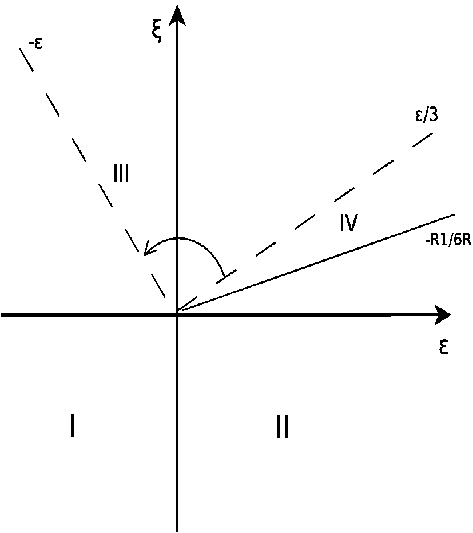
\includegraphics{./Diagram1.pdf}
 % Diagram1.pdf: 227x256 pixel, 72dpi, 8.01x9.03 cm, bb=0 0 227 256
 \caption{case:1}
 \label{fig:1}
\end{figure}


IV-2. $-R_1/2>R>0$ \\
The point describes by the same expressions (\ref{4-1}), but $\alpha$ changes from $\alpha_{0}$ to $\infty$,
where $\alpha_{0}=-5(R+R_1/2)/(R-R_1/6)>0$. In this case $-R1/6R>1/3$, and when $\alpha=0$, regions II and III
 are crossed (fig.[2]).

\begin{figure}
 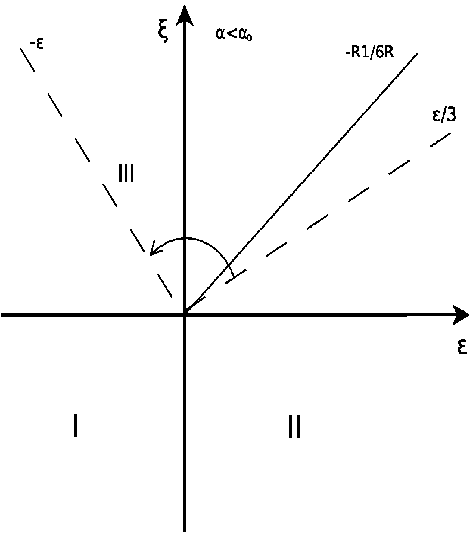
\includegraphics{./Diagram3.pdf}
 % Diagram3.pdf: 227x256 pixel, 72dpi, 8.01x9.03 cm, bb=0 0 227 256
 \caption{case:2}
 \label{fig:2}
\end{figure}


 When $\alpha$ grows boundaries of point II rotates counter clockwise and when $\alpha=\alpha_0$ boundaries of points II and III are coincides (fig.[3]).

\begin{figure}
 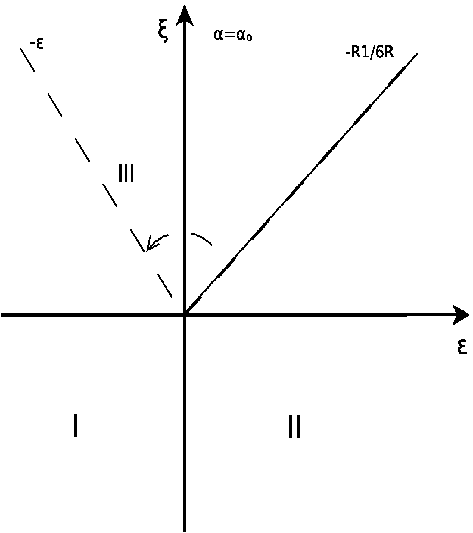
\includegraphics{./Diagram4.pdf}
 % Diagram4.pdf: 227x256 pixel, 72dpi, 8.01x9.03 cm, bb=0 0 227 256
 \caption{case:2}
 \label{fig:3}
\end{figure}

For $\alpha>\alpha_0$ regions II and III aren't crossed and between them we have IV regime like in the case 1 (fig.[4]).

\begin{figure}
 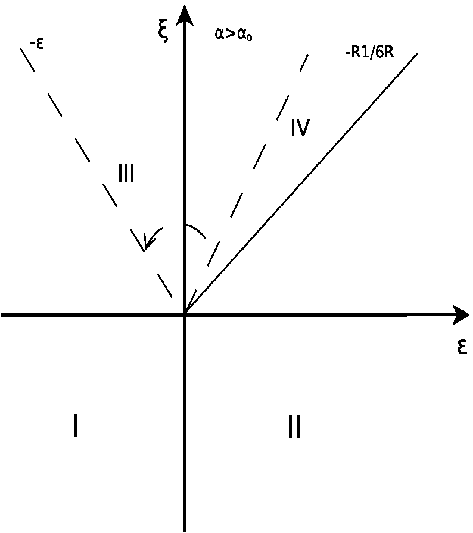
\includegraphics{./Diagram5.pdf}
 % Diagram5.pdf: 227x256 pixel, 72dpi, 8.01x9.03 cm, bb=0 0 227 256
 \caption{case:2}
 \label{fig:4}
\end{figure}

IV-3. $0>R>R_1/6$ \\
For this parameters we have no II regime.
In this case regime of stability IV point describes by this inequalities:
\begin{eqnarray}
\xi<\varepsilon(5+\alpha)/(15-\alpha),
\label{4case31}
 \\
 \xi<\varepsilon\frac{(5+\alpha)(R+R_1/6)}{(5-\alpha)2R},
\label{4case32}
\\
\alpha>\alpha_0.
\label{4case33}
\end{eqnarray}

But now $\alpha_0<0$ so the both inequalities (\ref{4case31}), (\ref{4case32}) are satisfied in a sector in the upperleft quadrant;
the lower bound is (\ref{4case31}) and the upper bound is (\ref{4case32}).
When $\alpha$ changes from $\alpha$ to $\infty$, the coefficient
in (\ref{4case31}) changes from $−R1/6R$ to $−(R + R1 /6)/2R$. The coefficient $(5+\alpha)/(15-\alpha)$ changes from $−R1/6R$ to $−1$. Thus for
$\alpha=\alpha_0$ the domain has zero width, and when $\alpha$ grows it is getting wider (fig.[5,6,7]).

\begin{figure}
 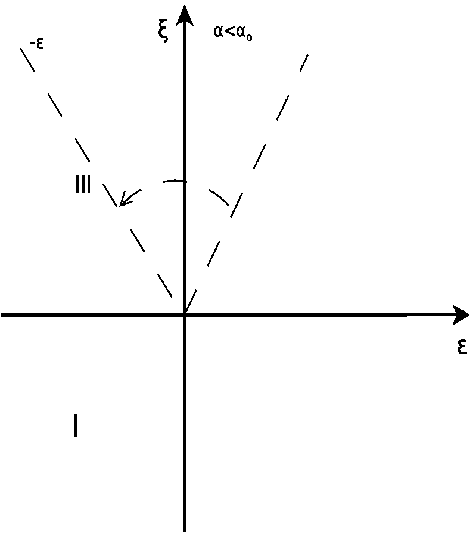
\includegraphics{./Diagram6.pdf}
 % Diagram7.pdf: 227x256 pixel, 72dpi, 8.01x9.03 cm, bb=0 0 227 256
 \caption{case3}
 \label{fig:5}
\end{figure}

\begin{figure}
 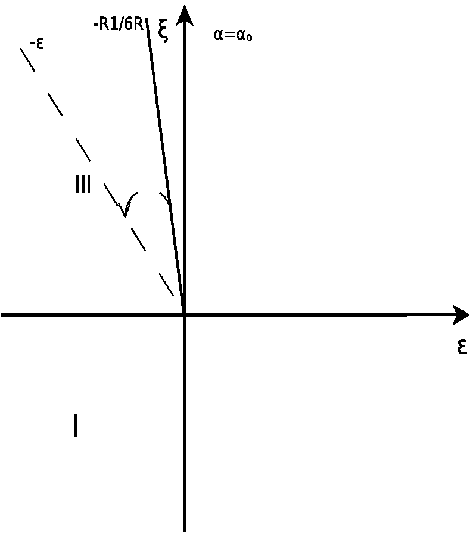
\includegraphics{./Diagram7.pdf}
 % Diagram7.pdf: 227x256 pixel, 72dpi, 8.01x9.03 cm, bb=0 0 227 256
 \caption{case:3}
 \label{fig:6}
\end{figure}

\begin{figure}
 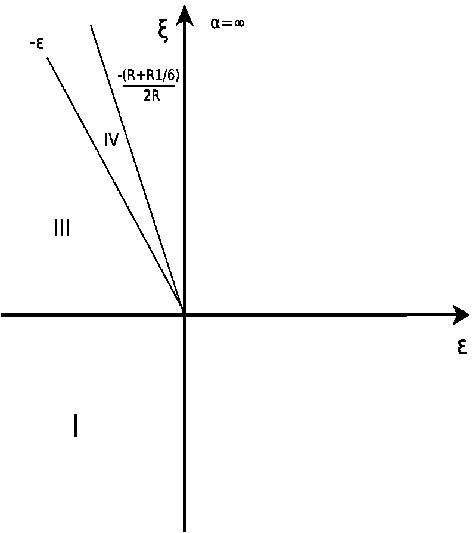
\includegraphics{./Diagram8.pdf}
 % Diagram8.pdf: 227x256 pixel, 72dpi, 8.01x9.03 cm, bb=0 0 227 256
 \caption{case:3}
 \label{fig:7}
\end{figure}




\section*{References}
\begin{thebibliography}{99}

\bibitem{Zinn} Zinn-Justin J 1989 {\it Quantum Field Theory and Critical
Phenomena} (Oxford: Clarendon)

\bibitem{Book3} Vasil'ev A N 2004 {\it The Field Theoretic Renormalization
Group in Critical Behavior Theory and Stochastic Dynamics}
(Boca Raton: Chapman \& Hall/CRC)

\bibitem{HH} Halperin B I and Hohenberg P C 1977 {\it Rev. Mod. Phys.}
{\bf 49} 435; Folk R and Moser G 2006 {\it J. Phys. A: Math. Gen.}
{\bf 39} R207

\bibitem{Hinr} Hinrichsen H 2000 {\it Adv. Phys.} {\bf 49} 815;
 \'Odor G 2004 {\it Rev. Mod. Phys.} {\bf 76} 663

\bibitem{JT} Janssen H-K and T\"{a}uber U C 2004 {\it Ann. Phys. (NY)}
{\bf 315} 147

\bibitem{Ivanov} Ivanov D Yu 2003 {\it Critical Behaviour of
Non-Idealized Systems} (Moscow: Fizmatlit) [in Russian]

\bibitem{quench} Khmel'nitski D E 1975 {\it Sov. Phys. JETP} {\bf 41} 981;
Shalaev B N 1977 {\it Sov. Phys. JETP} {\bf 26} 1204;
Janssen H-K, Oerding K and Sengespeick E 1995
{\it J. Phys. A: Math. Gen.} {\bf 28} 6073

\bibitem{Satten} Satten G and Ronis D 1985 {\it Phys. Rev. Lett.}
{\bf 55} 91; 1986 {\it Phys. Rev.} A {\bf 33} 3415

\bibitem{Onuki} Onuki A and Kawasaki K 1980 {\it Progr. Theor. Phys.}
{\bf 63} 122;
Onuki A, Yamazaki K and Kawasaki K 1981 {\it Ann. Phys.} {\bf 131} 217;
Imaeda T, Onuki A and Kawasaki K 1984 {\it Progr. Theor. Phys.} {\bf 71} 16

\bibitem{Beysens} Beysens D, Gbadamassi M and Boyer L 1979
{\it Phys. Rev. Lett} {\bf 43} 1253;
Beysens D and Gbadamassi M 1979 {\it J. Phys. Lett.} {\bf 40} L565

\bibitem{Ruiz} Ruiz R and Nelson D R 1981 {\it Phys. Rev.} A {\bf 23}
3224; {\bf 24} 2727;
Aronowitz A and Nelson D R 1984 {\it Phys. Rev.} A {\bf 29} 2012

\bibitem{AHH} Antonov N V, Hnatich M and Honkonen J 2006
{\it J. Phys. A: Math. Gen.} {\bf 39} 7867

\bibitem{Alexa} Antonov N V and Ignatieva A A 2006
{\it J. Phys. A: Math. Gen.} {\bf 39} 13593

\bibitem{AIK} Antonov N V, Iglovikov V I and Kapustin A S 2009
{\it J. Phys. A: Math. Theor.} {\bf 42} 135001

\bibitem{AIM} Antonov N V, Ignatieva A A and Malyshev A V 2010
E-print LANL arXiv:1003.2855 [cond-mat]; to appear in {\it PEPAN
(Phys. Elementary Particles and Atomic Nuclei, published by JINR)} {\bf 41}

\bibitem{FGV} Falkovich G, Gaw\c{e}dzki K and Vergassola M  2001
{\it Rev. Mod. Phys.} {\bf 73} 913

\bibitem{JphysA} Antonov N V 2006 {\it J. Phys. A: Math. Gen.} {\bf 39} 7825

\bibitem{Compress} Antonov N V, Hnatich M and Nalimov M Yu 1999
{\it Phys. Rev.} E {\bf 60} 4043

\bibitem{vanK} van Kampen N G 2007 {\it Stochastic Processes in Physics
and Chemistry, 3rd ed.} (Amsterdam: North Holland)

\bibitem{Sak} Sak J 1973 {\it Phys. Rev.} B {\bf 8} 281;
Honkonen J and Nalimov M Yu 1989 {\it J. Phys. A: Math. Gen.} {\bf 22} 751
Janssen H-K 1998 {\it Phys. Rev.} E {\bf 58} R2673;
Antonov N V 1999 {\it Phys. Rev.} E {\bf 60} 6691;
2000 {\it Physica} D {\bf 144} 370

\bibitem{Levy} Janssen H-K, Oerding K, van Wijland F and Hilhorst H J
1999 {\it Eur. Phys. J.} B {\bf 7} 137; Janssen H-K and Stenull O 2008
{\it Phys. Rev.} E {\bf 78} 061117

\end{thebibliography}
\end{document}



\bibitem{Bender} Bender C M, Brody D C and Jones H F 2004
{\it Phys. Rev. Lett.} {\bf 93} 251601

\bibitem{Pei} Peixoto M 1962 {\it Topology} {\bf 1} 101

\bibitem{Richt} Richtmyer R D 1981 {\it Principles of Advanced Mathematical
Physics, Vol.~2}  (Springer: NY)
